\subsection{CNN как векторизатор}

\begin{frame}{Дескрипторы классификационной CNN}

\begin{itemize}
    \item Свёрточные нейросети умеют правильно классифицировать картинки.
    \item Внутреннюю информацию можно извлечь и использовать в качестве описания картинки!
\end{itemize}

\centering
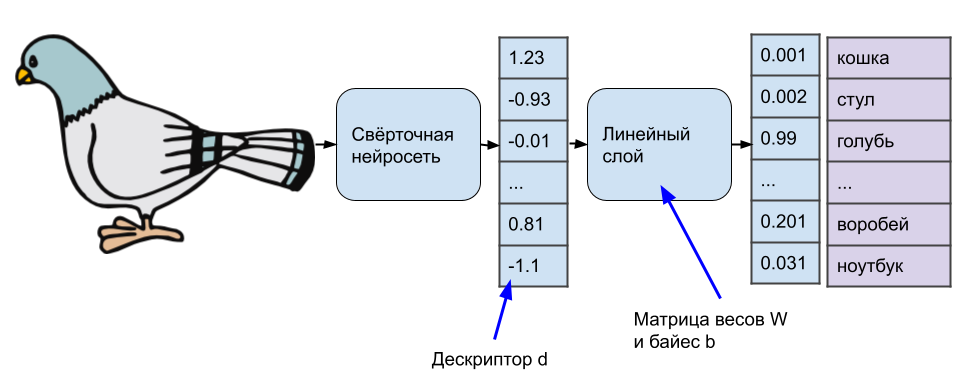
\includegraphics[width=0.8\textwidth]{images/pigeon CNN.png}

Итоговые предсказания класса $i$: $ \sigma_i(W^\Tr_i d + b_i) = \frac{\exp ( W^\Tr_i d + b_i )}{\sum_j \exp ( W^\Tr_j d + b_j )}$
    
\end{frame}

\begin{frame}{Вспоминаем задачу классификации}

Мы пытаемся минимизировать кроссэнтропию:
\[
CE(X,\,Y) = - \frac{1}{B} \sum_{k=1}^{B} \ln \frac{e^{W_{y_k}^\Tr d_k + b_{y_k}}}{ \sum_{j=1}^{N} e^{ W_{j}^\Tr d_k + b_{j} } } \rightarrow \min_{W,\,b,\,d}
\]

Сконцентрируемся только на одном объекте класса $i$:

\[
- \ln \frac{e^{W_{i}^\Tr d + b_i}}{ \sum_{j=1}^{N} e^{ W_{j}^\Tr d + b_{j} } } = 
\ln \left( \sum_{j=1}^{N} e^{ W_{j}^\Tr d + b_{j} } \right) - \ln e^{W_{i}^\Tr d + b_i} = 
\ln \left( \sum_{j=1}^{N} e^{ W_{j}^\Tr d + b_{j} } \right) - \left( W_{i}^\Tr d + b_i \right)
\]

Мы хотим, чтобы дескриптор $d$ был похож на столбец $W_i$ больше, чем на другие столбцы!
    
\end{frame}
